\chapter{Introduction}

\begin{flushright}
\begin{minipage}[t][0cm][b]{0.47\textwidth}
\emph{Se não podes entender, crê para que entendas. A fé precede, o intelecto segue.}
\end{minipage}

\rule[0cm]{7cm}{0.03cm}%{largura}{espessura}

Santo Agostinho
\end{flushright}

The Graph Theory is a branch of the math that is used by the computer science to describe and model several real and theoretical problems.  This doctoral thesis is dedicated to solving some problems of graph theory. In particular, in this chapter you will find a brief description of the related problems, the motivation of the study and a resume on the organization of the text.

\section{Motivation and Goals}

Um grafo EPG $G$ é um grafo que admite uma representação em que seus vértices são representados por caminhos de uma grade $Q$, tal que dois vértices de $G$ são adjacentes se e somente se os caminhos correspondestes tem no mínimo uma aresta em comum.

% The searches on path intersection graph are approached considering intersections from vertices or edges. Cases where models of intersection have a tree as host appear first in the literature e.g. \cite{gavril1974intersection, golumbic1985edge, golumbic1985}, later representations on a grid were considered, e.g. \cite{golumbic2009,golumbic2013, golumbic2013intersection}. More details on each intersection model will be given in the following text.

% The research of paths whose host is a tree starts in 1974 with Gavril~\cite{gavril1974intersection} who proved that a graph $G$ is an intersection graph of subtrees family of a tree if and only if $G$ is a chordal graph. An undirected graph $G$ is called an EPT graph if it is the edge intersection graph of a family of paths in a tree. Let $P$ be a family of paths on a host tree $T$ . Two types of intersection graphs from the pair $<P,T>$ are defined, namely VPT and EPT graphs.
% The \textit{edge intersection graph} of $P$, EPT(P), has vertices which correspond to the members of P, and two vertices are adjacent in EPT(P) if and only if the corresponding paths in P share at least one edge in T. Similarly, the \textit{vertex intersection graph} of P, VPT(P), has vertices which correspond to the members of P, and two vertices are adjacent in VPT(P) if and only if the corresponding paths in P share at least one vertex in T.

% VPT and EPT graphs are incomparable families of graphs. However, when the maximum degree of the host tree is restricted to 3 the family of
% VPT graphs coincides with the family of EPT graphs, \cite{alcon2010necessary}.

%  Golumbic, Lipshteyn and Stern defined in 2009 the class of EPG graphs, as the  intersection graph of edge paths on a grid. An EPG graph $G$ is a graph that admits a representation where its vertices correspond to paths in a grid $Q$, such that two vertices of $G$, we say $v_1$ and $v_2$, they are adjacent if and only if their corresponding paths $P_{v_1}$ and $P_{v_2}$, they have a common edge in $Q$. If the paths in the representation have at most $k$ changes of direction  (bends), we say that it is a  $B_k$-EPG representation. In particular when the paths of this representation have at most 1 bend we say that this is a $B_1$-EPG representation or single bend representation for EPG graphs.  A collection $C$ of sets satisfies the Helly property when every sub-collection of $C$ that is pairwise intersecting has at least one common element. 




O estudo de grafos EPG tem motivação relacionada com o problema de \textit{design} VLSI que combina a noção de grafos de intersecção de arestas de caminhos em uma árvore com um modelo de \textit{layout} de grade VLSI~\cite{golumbic2009}. O número de dobras em um circuito integrado pode aumentar a área de \textit{layout} e consequentemente aumentar o custo de produção do microchip. 
Essa é uma das principais aplicações que instigam a  pesquisa sobre representações EPG de algumas famílias de grafos quando existem restrições no número de dobras nos caminhos usados na representação.
Outras aplicações e detalhes sobre problemas de \textit{layout} de circuitos podem ser encontrados em~\cite{bandy1990, molitor1991}.   

Um grafo é $ B_k$-EPG se ele admite uma representação (sobre uma grade) em que cada caminho possua no máximo $k$ dobras. A título de exemplo a Figura~\ref{fig:trianguloepgRepresentacao}(a) retrata um grafo $C_3$, a Figura~\ref{fig:trianguloepgRepresentacao}(b) retrata uma representação EPG do grafo $C_3$ onde os caminhos não possuem dobra e a  Figura~\ref{fig:trianguloepgRepresentacao}(c) retrata uma representação com 1 dobra do grafo $C_3$. Consequentemente, $C_3$ é um grafo  $B_0$-EPG. %De forma mais geral, grafos $B_0$-EPG coincidem com grafos de intervalo~\cite{golumbic2009}.

O \emph{número de dobras} de uma classe de grafos é o menor  $k$ para o qual todos os grafos na classe possuem uma representação $B_k$-EPG. Grafos de intervalo possuem número de dobras $0$~\cite{golumbic2009}, árvores possuem  número de dobras $1$~\cite{golumbic2009} e  grafos outerplanar possuem número de dobras $2$~\cite{daniel2014b}. O número de dobras da classe dos grafos planares é um problema em aberto, porém sabe-se que ele é $ 3 $ ou $4$~\cite{daniel2014b}. %Apesar de existirem demonstrações de que o número de dobras não é maior que 4 para a classe dos grafos planares, também não se conhece algum grafo planar que não possa ser representado com 3 dobras.

A classe dos grafos EPG tem sido estudada em diversos trabalhos, tais como  \cite{alcon2016, Asinowski2009, cohen2014, golumbic2009, heldt2014,  martin2017}, entre outros. As investigações frequentemente abordam caracterizações com relação número de dobras das representações de um grafo. A respeito da complexidade de reconhecimento de grafos $B_k$-EPG, somente a complexidade de reconhecimento de três subclasses de grafos EPG foi determinada:
 grafos $B_0$-EPG podem ser reconhecidos em tempo polinomial, uma vez que correspondem a classe de grafos de intervalo, ver~\cite{booth1976, golumbic2009}. Em contraste, o reconhecimento das classes $B_1$-EPG e $B_2$-EPG é $NP$-completo, ver~\cite{heldt2014, martin2017}.

\begin{figure}[h]
  \centering
  \begin{tabular}{ c p{0.15cm} c p{0.15cm} c }
    %\centering
    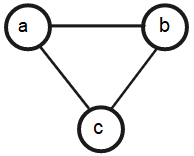
\includegraphics[width=2.3cm]{./img/trianguloabc.png} && 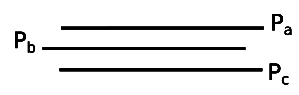
\includegraphics[width=4cm]{./img/edge-clique.png} & &
    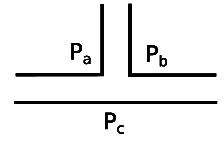
\includegraphics[width=3.3cm]{./img/claw-clique.png}
    \\
    \footnotesize %\centering 
    (a) O grafo $C_3$ && \footnotesize(b) Representação $B_0$-EPG de $C_3$ && \footnotesize (c) Representação $B_1$-EPG de $C_3$\\

  \end{tabular}

 \caption{O grafo $ C_3 $ com duas representações, uma sem dobra e outra com uma dobra} \label{fig:trianguloepgRepresentacao}
\end{figure}


%A  collection $C$ of sets satisfies the Helly property when every sub-collection of $ C $ that is pairwise intersecting has at least one common element. The Helly property has this name in honor of the great Austrian mathematician Eduard Helly, who in 1923 proposed his famous theorem concerning the relation of intersecting sets.

%The study of the Helly property is useful in very diverse areas of science, and we can enumerate applications in semantics, code theory, computational biology, database, image processing, graph theory, optimization, and linear programming \cite{dourado2009}.

%Note that the representation of Figure~\ref{fig:trianguloepgRepresentacao}(b) satisfies the Helly property, while the representations of Figures~\ref{fig:trianguloepgRepresentacao}(c) and~\ref{fig:trianguloepgRepresentacao}(d) do not satisfy it.

Este trabalho propõe o estudo de grafos que possuem uma representação EPG-Helly. 
A propriedade Helly relacionada com representações EPG foi  estudada em~\cite{golumbic2009} e \cite{golumbic2013}. Em particular, esses trabalhos determinaram um parâmetro conhecido como número de Helly forte  para grafos $B_1$-EPG. 

Estão no escopo de interesse deste trabalho os seguintes tópicos:

\begin{itemize}
    
    \item Determinar a complexidade de reconhecimento de grafos $B_1$-EPG-Helly;
    \item Determinar limites superiores e/ou inferiores para os parâmetros número de Helly e número de Helly forte em grafos EPG e EPG-Helly;
    
    \item Estudar os parâmetros número de Helly e número de Helly forte também em grafos de intersecção de vértices em caminhos sobre grade (VPG e VPG-Helly);
    
    \item Estudar o relacionamento entre as classes de grafos EPT, VPT e $B_1$-EPG.
    
\end{itemize}



% \section{Motivação}
% Por que pesquisar?

% Qual a relevância do problema e por que escolher esse tema?

% Qual é o problema estudado?
% Onde ele acontece?
% Quem observou ou observa sua ocorrência?
% Por que isso é importante e deve ser solucionado?

% \section{Objetivo}

% Quais as finalidades intelectuais?

% verificar... compreender... analizar...
% comparar...

\section{Organization of the thesis}

No Capítulo 2 apresentaremos algumas definições básicas sobre grafos juntamente com uma breve explicação sobre a propriedade Helly. Além disso, o capítulo aborda uma breve discussão sobre problemas de caminhos em grade.

O Capítulo 3 será dedicado à definição do problema estudado, análise de algumas representações EPG básicas e demonstração da $NP$-completude do problema de reconhecimento de grafos $B_1$-EPG-Helly. São publicações resultantes desta pesquisa, os seguintes escritos:

\begin{enumerate}
    \item BORNSTEIN, C. F.; SANTOS, T. D.; SOUZA, U. S.; SZWARCFITER, J. L. A Complexidade do Reconhecimento de Grafos B1-EPG-Helly. In: 50º SBPO - Simpósio Brasileiro de Pesquisa Operacional, 2018, Rio de Janeiro. Cidades Inteligentes: Planejamento Urbano, Fontes Renováveis e Distribuição de Recursos, 2018.

     \item BORNSTEIN, C. F.; SANTOS, T. D.; SOUZA, U. S.; SZWARCFITER, J. L. Sobre a Dificuldade de Reconhecimento de Grafos B1-EPG-Helly. In: XXXVIII Congresso da Sociedade Brasileira de Computação, 2018, Natal - RN. Computação e Sustentabilidade, 2018. p. 113-116.

     
     \item BORNSTEIN, C. F.; SANTOS, T. D.; SOUZA, U. S.; SZWARCFITER, J. L. The complexity of B1-EPG-Helly graph recognition. In: VIII Latin American Workshop On Cliques in Graphs (LAWCG), ICM 2018 Satellite Event, 2018, Rio de Janeiro. Program and Abstracts, 2018. p. 69.

     
     \item BORNSTEIN, C. F.; GOLUMBIC, M.C.; SANTOS, T. D.; SOUZA, U. S.; SZWARCFITER, J. L.  The complexity of B1-EPG-Helly graph recognition. %In:  45th International Workshop on Graph-Theoretic Concepts in Computer Science,  2019, Vall de Núria, Catalonia, Spain. 
     (Submited).
     
\end{enumerate}


Por fim, no Capítulo 4, discutimos os principais resultados obtidos para grafos EPG. Adicionalmente, teremos
também as considerações finais sobre o trabalho aqui apresentado com algumas perspectivas e ideias sobre o problema e possíveis direcionamentos para novos estudos de trabalhos futuros.